\documentclass[a4paper,12pt]{article}

\usepackage{cmap}
\usepackage{amsmath}
\usepackage[T2A]{fontenc}
\usepackage[utf8]{inputenc}
\usepackage[english,russian]{babel}
\usepackage{graphicx}



\title{Разработка системы управления колесным роботом}
\author{}
\begin{document}
\maketitle

\section{Задача управления колесным роботом}	

Колесная техника широко используется для решения различного рода задач. Способность траспортных средств к автономному движению может позволить повысить эффективность и безопасность эксплуатации машин, а также снизить затраты.

\subsection{Общая кинематическая схема колесного робота}

Конструкция робота включает в себя корпус, содержащий две колесных оси, принадлежащих одной плоскости. Скорость вращения задних колес определяет скорость движения робота. Передние колеса могут ограниченно поворачиваться вокруг вертикальной оси, определяя локальную кривизну траектории.


\subsection{Системы координат}

Положение колесного робота $r$ описывается положением начала связанной с роботом подвижной системы координат $B$ в некоторой локальной системе координат $I$, ось $Z_I$ направлена по гравитации, оси $X_I$ и $Y_I$ дополняют систему до правой тройки.

Система координат $B$ связана с серединой задней оси робота, при этом  ось $X_B$ направлена к середине передней оси робота, ось $Y_B$ лежит в плоскости платформы и направлена вправо, ортогонально $X_B$, $Z_B$ дополняет систему до правой тройки.

Ориентация робота представлена кватернионом $q = (q_0 \quad \textbf{q})^T$ таким образом, что произвольный вектор, записанный в собственных осях $B$ робота проецируется в локальную систему как
$r_I = q_{IB} \circ r_B \circ \tilde{q}_{IB}$.

Кватернион ориентации эквивалентен матрице поворота
\begin{equation} \label{eq:quat_to_rotmx}
C = ({q_0}^2 -  \textbf{q}^T  \textbf{q}) E_{3 \times 3} + 2  \textbf{q}^T  \textbf{q} - 2 {q_0} [ \textbf{q}]_{\times},
\end{equation}
где $E_{n \times n}$ -- едичная матрица размерности $n$, $[...]_{\times}$ -- оператор векторного произведения:

\begin{equation} \label{eq:cross_operator}
[{\textbf{q}}]_{\times} =
\begin{bmatrix}
0            & -{\textbf{q}}_z   & {\textbf{q}}_y \\
{\textbf{q}}_z     & 0           &-{\textbf{q}}_x\\
-{\textbf{q}}_y    & {\textbf{q}}_x    & 0
\end{bmatrix}.
\end{equation}

РИСУНОК ОБЩИЙ ВИД РОБОТА И СИСТЕМЫ КООРДИНАТ

\subsection{Модель движения робота}
Движение робота определяется его текущей ориентацией и управляющим воздействием на приводы колес $v$.
\begin{align} \label{eq:model_velocity}
&\dot{r}_B = v e_B = (v \quad 0 \quad 0)^T \\
&\dot{r}_I = v (q_{IB} \circ e_B \circ \tilde{q}_{IB}) =
v e_I
\end{align}

Вектор угловой скорости робота $\Omega_B = (\omega_x \quad \omega_y \quad \omega_z)^T$ связан с кватернионом ориентации уравнением Пуассона
\begin{align}  \label{eq:model_rot_velocity}
&\dot{q}_{IB} = \frac{1}{2} q_{IB} \circ \Omega_{B}
\end{align}
Изменение ориентации робота определяется поворотом руля $u$
\begin{align}  \label{eq:model_rot_velocity_z}
&\omega_{z} = vu
\end{align}
и, в случае движения по неровной поверхности, изменением ее наклона.

\subsection{Обеспечение движения робота по целевой траектории}
Целью управления является обеспечение движения робота по известной заранее траектории.  Целевая траектория принадлежит поверхности и задана явно в параметрической форме $p(s)$, где $p(s)$ -- дважды непрерывно дифференцируемая функция, а $s$ -- длина дуги кривой.


\section{Синтез системы управления колесным роботом}

\subsection{Плоское движение колесного робота}
Синтез контура управления робота для плоского движения колечного робота 

\subsection{Движение робота по криволинейной поверхности}

Обозначим $\Delta$ -- вектор смещения робота
\begin{align}  \label{eq:Delta}
&\Delta = r - p(s^*),
\end{align}
где $p(s^*)$ -- это ближайшая к роботу точка на целевой траектории:
\begin{align}\label{eq:ort}
&\Delta^T p'(s^*) = 0.
\end{align}
Обозначим $\delta$ -- расстояние до целевой траектории
\begin{align}  \label{eq:delta}
&\delta = \sqrt{\Delta^T \Delta}
\end{align}
Тогда,
\begin{align}  \label{eq:delta_dot}
&\dot \delta = \frac{\Delta^T \dot \Delta}{\delta} = \frac{\Delta^T (ve_I - p'(s^*) \dot {s^*})}{\delta} = 
\frac{v \Delta^T e_I}{\delta}.
\end{align}

В качестве независимой переменной выберем
$\xi$ длину пути, пройденного роботом, тогда 
\begin{align}  \label{eq:xi_dot}
&\dot \xi = v.
\end{align}
В качестве фазовой переменной выберем расстояние
$z_1 = \delta$,
тогда, с учетом \eqref{eq:delta_dot}, \eqref{eq:xi_dot}
\begin{align}  \label{eq:z1_dxi}
&(z_1)_{\xi} = \frac{\dot \delta}{\dot \xi} = \frac{\Delta^T }{\delta} e_I = \cos \varphi, 
\end{align}
где $\varphi$ -- угол между направлением на ближайшую точку целевой траектории
\begin{align}  \label{eq:d_I}
&d_I = \frac{\Delta }{\delta}, 
\end{align}
и направлением скорости робота $e_I$.
Обозначим $z_2 = \cos \varphi$, тогда

\iffalse
\begin{align}  \label{eq:z2_dxi_phi}
&(z_2)_{\xi} = -\sin \varphi \frac{\dot \varphi}{\dot \xi}
\end{align}
\fi


\begin{align}  \label{eq:z2_dxi}
&(z_2)_{\xi} = \frac{d_I^T \dot e_I + \dot d_I^T  e_I}{\dot \xi}.
\end{align}
Здесь
\begin{align}  \label{eq:e_I_dot}
&\dot e_I = \Omega_{B} \times e_I = [\Omega_{B}]_{\times} e_I,
\end{align}

\begin{align}  \label{eq:d_I_dot}
&\dot d_I = \frac{\dot \Delta}{\delta} - \frac{\Delta }{\delta^2} \dot \delta = \frac{\dot \Delta}{\delta} - \frac{v \Delta \cos \varphi}{\delta^2}.
\end{align}
Тогда
\begin{align}  \label{eq:z2_dxi_2}
&(z_2)_{\xi} =\frac
{d_I^T [\Omega]_{\times} + \frac{\dot \Delta^T}{\delta}}
{v} e_I -
\frac{\cos^2 \varphi }{\delta}
.
\end{align}

\begin{align}  \label{eq:z2_dxi_3}
&(z_2)_{\xi} =
\frac{d_I^T [\Omega]_{\times} e_I}{v} +
\frac{\dot \Delta^T e_I}{\delta v} -
\frac{\cos^2 \varphi }{\delta}
.
\end{align}

\iffalse
\begin{align}  \label{eq:z2_dxi_22}
&(z_2)_{\xi} = \frac{
	d_I^T [\Omega_{B}]_{\times} e_I +
	\frac{\dot \Delta^T}{\delta} e_I
}
{v}
- \frac{\Delta^T \cos \varphi}{\delta^2} = \\
& =\frac{
	\Delta^T [\Omega_{B}]_{\times} +
	\dot \Delta^T 
}
{v \delta} e_I
- d_I^T \cos^2 \varphi
\end{align}
\fi

...

\subsection{Обеспечение обратных связей в контуре управления}
Для реализации закона управления необходимо иметь обратную связь по текущему положению, скорости, ориентации и угловой скорости робота.

Для прямых измерений положения и скорости робота используется приемник сигналов глобальной навигации. Измерения угловой скорости производятся датчиком угловой скорости. Ориентация робота может быть однозначно определена с помощью двух дополнительных приемников сигналов глобальной навигации, а также в одноантенном варианте, с использованием модели движения робота без проскальзывания в расширенном фильтре Калмана. Для повышения качества оценки состояния дополнительно используются показания датчика линейного ускорения.

В качестве алгоритма фильтрации выбрана квадратно-корневая реализация расширенного фильтра Калмана(SR-EKF). Вектор состояния составлен из положения, скорости, ускорения, кватерниона ориентации и угловой скорости
\begin{align} 
&x = (r_I \quad \dot{r}_I \quad \ddot{r}_I \quad q_{IB} \quad \Omega_B)
\end{align}

На первом этапе работы алгоритма производится априори оценка текущего состояния на основе предыдущей оценки и модели движения
\begin{align}
x_k^- = f(x_{k-1}, \delta t).
\end{align} 
Квадратный корень ковариации априори оценки состояния определяется как
\begin{align}
\begin{split}
&\sqrt{P^-_k} = \Big[ (E_{n \times n} +  F_k \delta t) \sqrt{P_{k-1}} \quad Q \sqrt{\delta t}  \Big] \Theta,
\end{split}
\end{align}
где $\Theta$ -- ортогональное преобразование, приводящее левую часть к нижнему треугольному виду. Здесь
\begin{align}
\begin{split}
&F = \frac{f(x,t)}{\delta x}.
\end{split}
\end{align}

На этапе коррекции находим скорректированную ковариацию оценки и измерений, а также коэффициент усиления
\begin{align}
\begin{pmatrix}
&\sqrt{R_k} &0 \\
&K_k &\sqrt{P_k}
\end{pmatrix}
=
\begin{pmatrix}
&\sqrt{R} &H_k \sqrt{P_k^-} \\
&0 &\sqrt{P_k^-},
\end{pmatrix} \Theta
\end{align}
где $H_k$ -- линеаризованная функция измерений  
\begin{align}
\begin{split}
&H_k = \frac{\delta h(x_k^-)}{\delta x}
\end{split}
\end{align}
Оценка состояния
\begin{align}
\begin{split}
&x_k = x_k^- + K_k * (\sqrt{R_k})^{-1} \big(z_k - h(x_k^-)\big)
\end{split}
\end{align}

Таким образом, априори оценка состояния определяется на основе интегрирования показаний датчиков линейного ускорения и угловой скорости: 
\begin{align} \label{eq:rddot_i_calib}
\begin{split}
&\ddot{r}_{I} = {q}_{IB} \circ  a^{imu} \circ \tilde{q}_{IB} + g_I \\
&\Omega_B = w^{\textit{gyr}} \\
\end{split}
\end{align}

Для коррекции используются показания систем глобальной навигации
\begin{align}
z_1 = (r^{gnns} \quad v^{gnns}).
\end{align}

\begin{align}
\begin{split}
&H_1 =
\begin{pmatrix}
E_{3x3} & O_{3x3} & O_{3x3} & Z^r_q & O_{3x3}   \\
O_{3x3} & E_{3x3} & O_{3x3} & Z^v_q & Z^v_{\Omega}
\end{pmatrix}
\end{split}
\end{align}
Здесь
\begin{align}
\begin{split}
&Z^r_q = [q_{IB} \circ \delta r^{gnns}_B \circ \tilde{q}_{IB}]_{ q_{IB}} \\
&Z^v_q = [q_{IB} \circ  (\Omega_B \times \delta r^{gnns}_B) \circ \tilde{q}_{IB}]_{ q_{IB}} \\
&Z^v_\Omega = [q_{IB} \circ  (\Omega_B \times \delta r^{gnns}_B) \circ \tilde{q}_{IB}]_{ \Omega_B}.
\end{split}
\end{align}

Также, используя модель движения без проскальзывания, можно записать
\begin{align}
\begin{split}
&v^{gnns} = v_I + q_{IB} \circ  (\Omega_B \times \delta r^{gnns}_B) \circ \tilde{q}_{IB} = \\
& = q_{IB} \circ (|v_I| \quad 0 \quad 0)^T \circ \tilde{q}_{IB} + q_{IB} \circ  (\Omega_B \times \delta r^{gnns}_B) \circ \tilde{q}_{IB}
\end{split}
\end{align}
Тогда, 
\begin{align}
z_2 = v^{gnns}.
\end{align}
\begin{align}
\begin{split}
&H_2 =
\begin{pmatrix}
O_{3x3} & \zeta^v_v & O_{3x3} & \zeta^v_q + Z^v_q & Z^v_{\Omega},
\end{pmatrix}
\end{split}
\end{align}
где
\begin{align}
\begin{split}
&\zeta^v_v = [q_{IB} \circ (|v_I| \quad 0 \quad 0)^T \circ \tilde{q}_{IB}]_{ v_I} \\
&\zeta^v_q = [q_{IB} \circ (|v_I| \quad 0 \quad 0)^T \circ \tilde{q}_{IB}]_{ q_{IB}}
\end{split}
\end{align}

Кроме этого, для коррекции могут использоваться показания датчиков линейного ускорения:
\begin{align} 
\begin{split}
&a^{imu}  = \tilde{q}_{IB} \circ (\ddot{r}_{I} - g_I) \circ q_{IB}
\end{split}
\end{align}
Тогда, 
\begin{align}
z_3 = a^{imu}
\end{align}
\begin{align}
\begin{split}
&H_3 =
\begin{pmatrix}
O_{3x3} & O_{3x3} & \alpha^{\ddot{r}}_a & \alpha^a_q & O_{3x3},
\end{pmatrix}
\end{split}
\end{align}
где
\begin{align}
\begin{split}
&\alpha^{\ddot{r}}_a = [\tilde{q}_{IB} \circ (\ddot{r}_{I} - g_I) \circ q_{IB}]_{ \ddot{r}_I} \\
&\alpha^a_q = [\tilde{q}_{IB} \circ (\ddot{r}_{I} - g_I) \circ q_{IB}]_{ {q}_{IB}}
\end{split}
\end{align}

\section{Программная реализация алгоритмов управления колесным роботом}
Для проверки предложенных алгоритмов они реализованы в виде отдельных программных модулей. Кроме этого созданы виртуальные модели и среда, модели измерений датчиков для проведения численных экспериментов. 

\subsection{Общая схема программной реализации системы управления роботом}
Ниже представлена общая схема программной реализации разработанных алгоритмов.
\begin{figure}[h!]
	\centering
	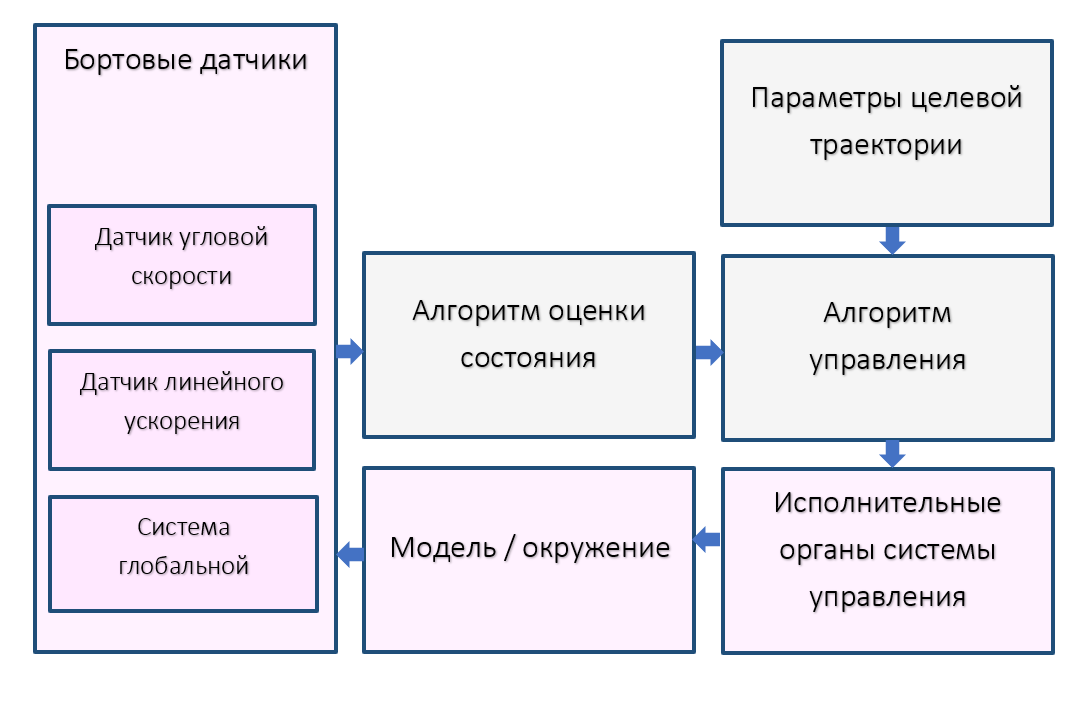
\includegraphics[width=10cm,clip]{pic/common_code_scheme}
	\caption{Общая схема программной реализации}
	\label{pic:common_code_scheme}
\end{figure}

\subsection{Реализация алгоритмов управления на базе ROS и Gazebo}
За основу для проектирования системы взят широко используемый в роботехнике пакет с открытым исходным кодом ROS (Robot Operating System). Ключевой особенностью ROS является использование распределенной архитектуры на основе графов, когда каждый программный модуль ROS (ROS Node) является изолированной частью системы и взаимодействует с другими ROS Node посредством сообщений, реализующих систему издатель-подписчик.

Для моделирования и визуализации используется программа с открытым исходным кодом для моделирования робототехнических систем Gazebo.

За основу одной из управляемых моделей колесного робота выбрана модель робота Husky.
\begin{figure}[h!]
	\centering
	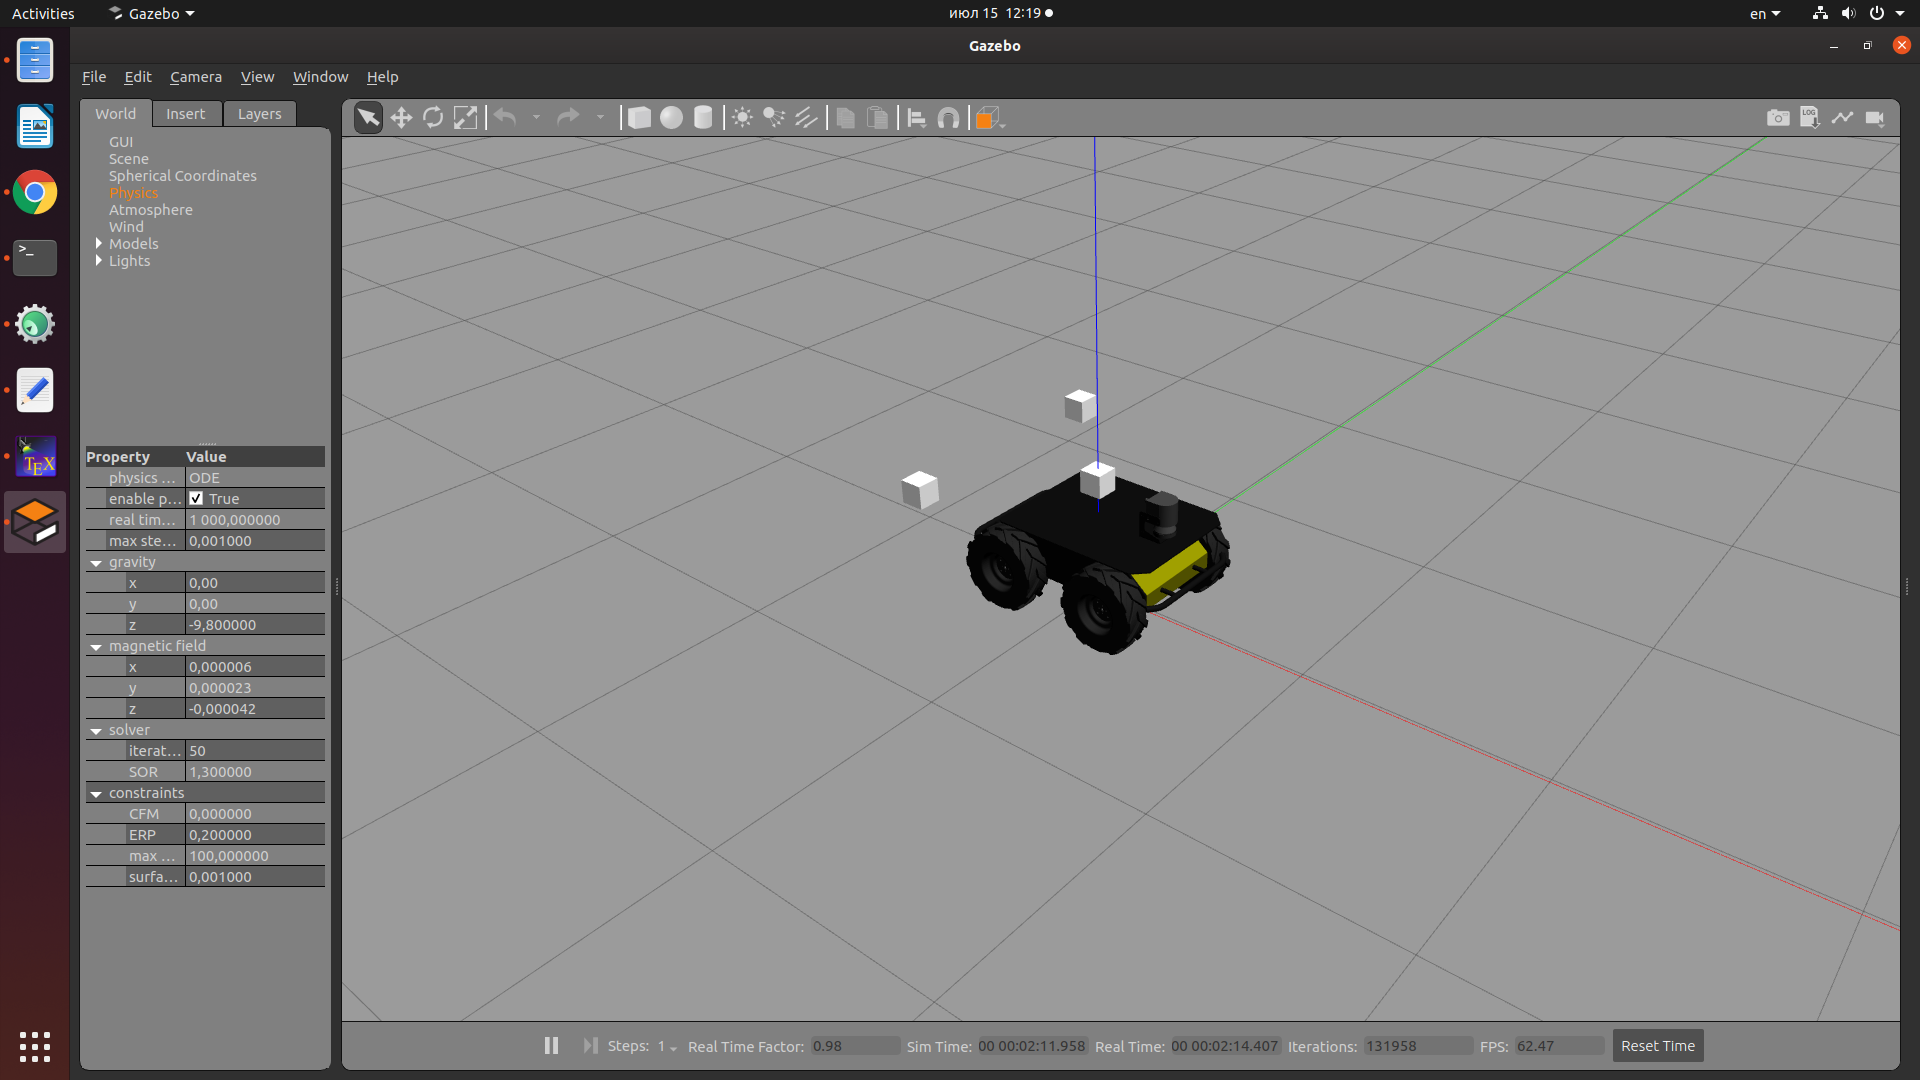
\includegraphics[width=14cm,clip]{pic/husky_gazebo}
	\caption{Визуальная модель Husky}
	\label{pic:husky_gazebo}
\end{figure}
\begin{figure}[h!]
	\centering
	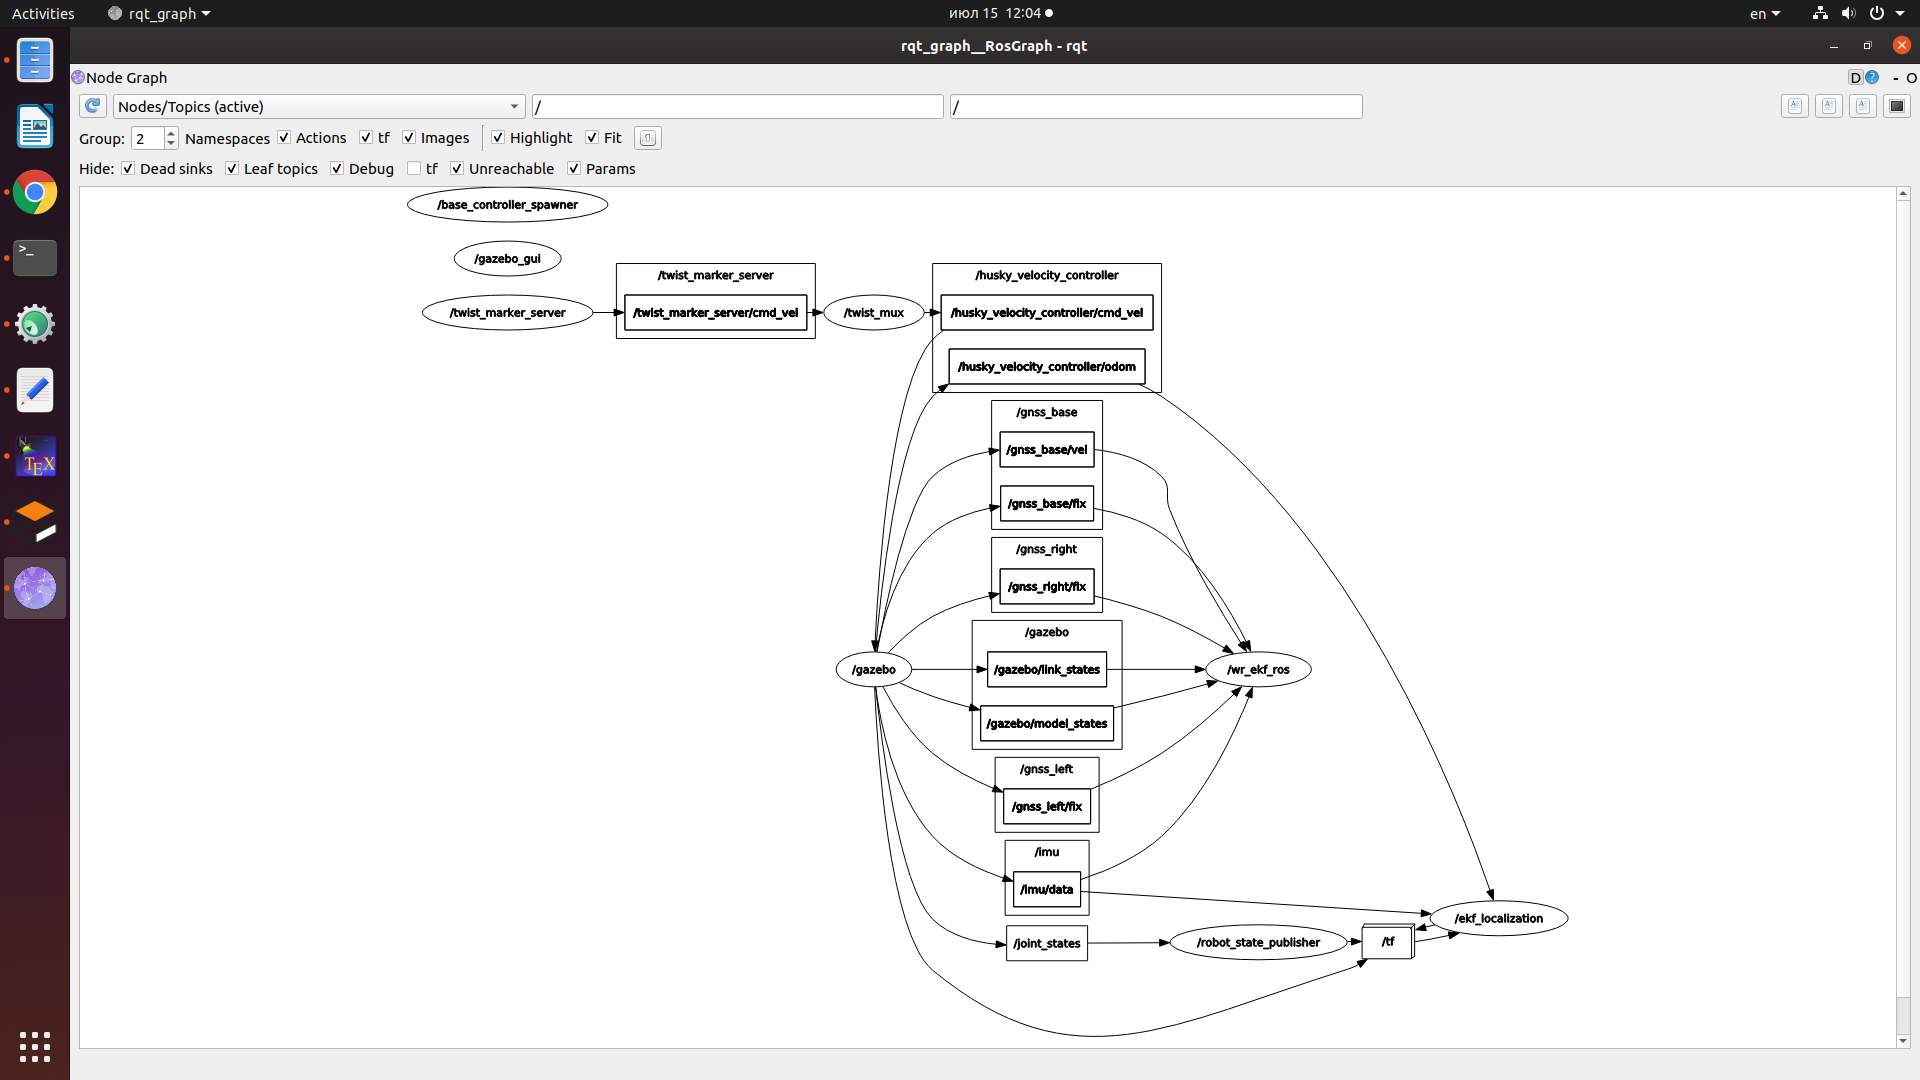
\includegraphics[width=14cm,clip]{pic/husky_rqt_plot}
	\caption{Граф подсистем Husky}
	\label{pic:husky_rqt_plot}
\end{figure}
В структуру подсистем Husky добавлены алгоритмы моделирования показаний бортовых датчиков, алгоритмы фильтрации и алогоритм управления на плоской поверхности.

Для отработки алгоритмов управления на неровной поверхности создана кинематическая модель движения робота по трехмерной поверхности без проскальзывания. Для визуалиции используется отцифрованная модель прототипа колесного робота, учавствующего в полевых экспериментах.

\begin{figure}[h!]
	\centering
	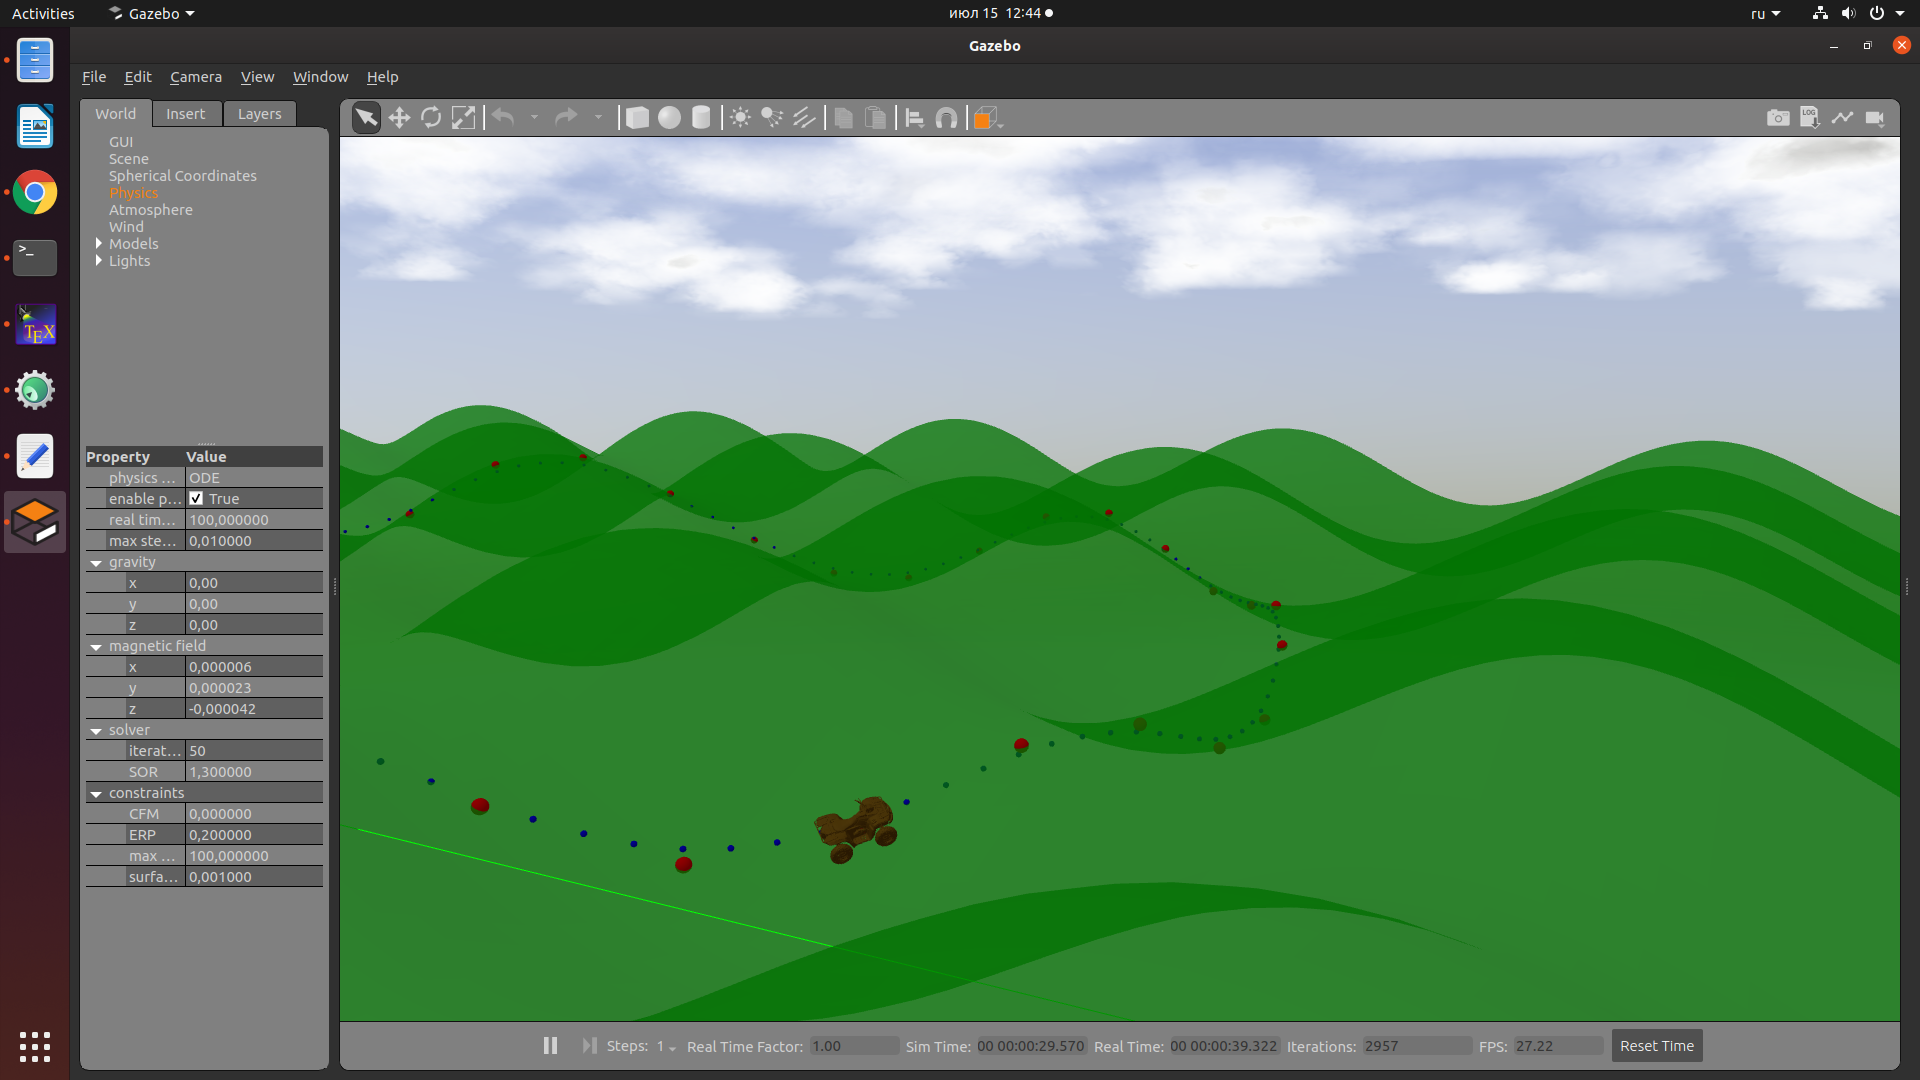
\includegraphics[width=14cm,clip]{pic/kin_gazebo}
	\caption{Визуальная модель колесного робота}
	\label{pic:kin_gazebo}
\end{figure}

\begin{figure}[h!]
	\centering
	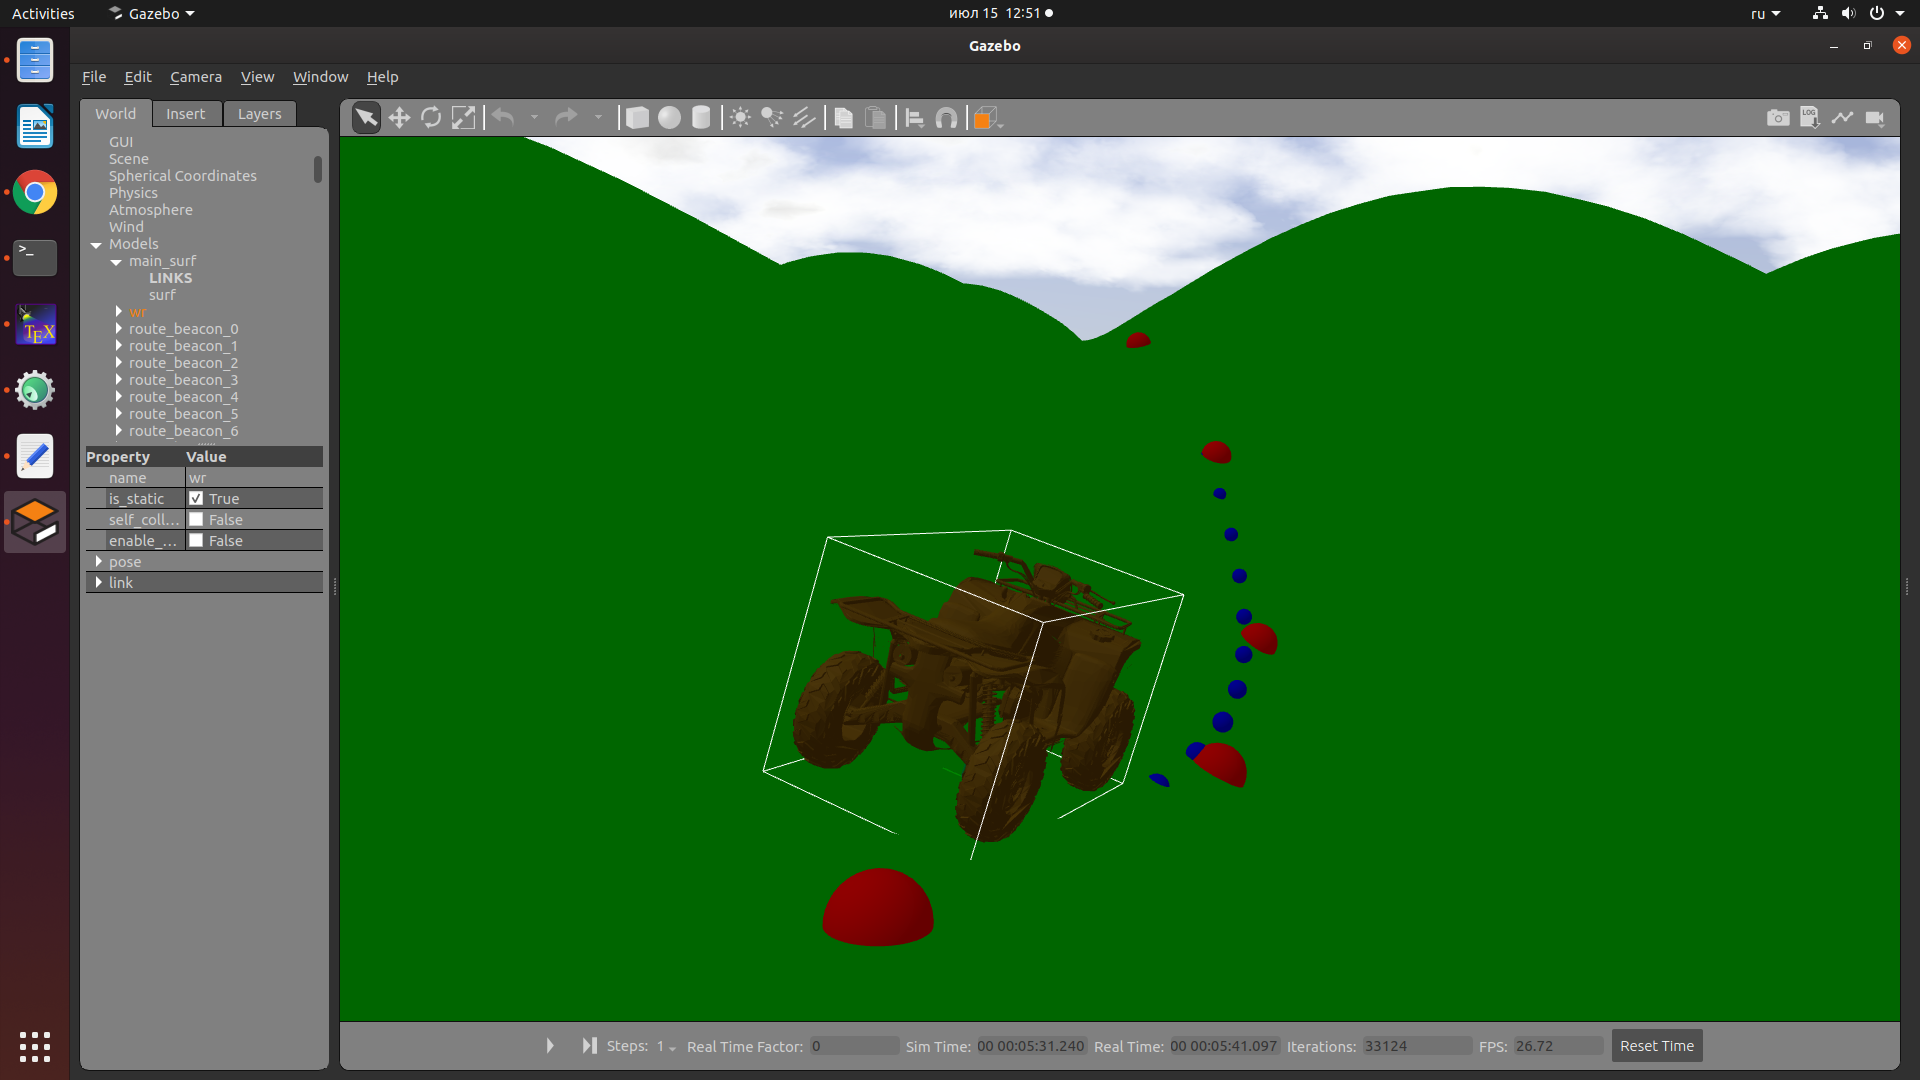
\includegraphics[width=14cm,clip]{pic/kin_gazebo2}
	\caption{Визуальная модель колесного робота}
	\label{pic:kin_gazebo2}
\end{figure}


\section{Прототипирование колесного робота}
\subsection{Исследовательский образец колесного робота}
Про машинку: общий вид, чертежи и схемы
\subsection{Цифровая модель робота в среде Gazebo}
Про перенос модели в Gazebo
\subsection{Эксперименты}
описание экспериметов


\section{}

\end{document}